\documentclass[pdftex,twocolumn,10pt,letterpaper]{article}
\usepackage{graphicx, subfigure, multirow, times}
\usepackage{url, amsfonts, verbatim, mathtools, color, soul}
\usepackage[small,compact]{title sec}
\usepackage{usenix}

\renewcommand{\ttdefault}{cmtt}
\usepackage{mdwlist}


\newenvironment{myitemize}
{
   \vspace{0mm}
    \begin{list}{$\bullet$ }{}
        \setlength{\topsep}{0em}
        \setlength{\parskip}{0pt}
        \setlength{\partopsep}{0pt}
        \setlength{\parsep}{0pt}
        \setlength{\itemsep}{1mm}
}
{
    \end{list}
}

\newcommand{\todo}[1]{\textbf{\textcolor{red}{TODO: #1}}}

% To make the FIXMEs go away, comment out this line...
\newcommand{\allnotes}[1]{}
% To make the FIXMEs go away, comment out this line...
\renewcommand{\allnotes}[1]{\textit{#1}}
\newcommand{\fixme}[1]{\allnotes{\bf\textcolor{red}{[#1]}}}
\newcommand{\panda}[1]{\allnotes{\bf\textcolor{blue}{[Panda: #1]}}}
\definecolor{comment-red}{rgb}{1,0,0}
\newcommand{\kay}[1]{\allnotes{\textnormal{\color{comment-red}{\textbf{KAY:#1}}}\unskip}}
\newcommand{\eat}[1]{}

\begin{document}
\title{\large \bf The Case for Tiny Tasks in Compute Clusters}
\author{
{\rm Kay Ousterhout$^*$, Aurojit Panda$^*$, Joshua Rosen$^*$, Shivaram Venkataraman$^*$, Reynold Xin$^*$}\\
\rm{Sylvia Ratnasamy$^*$, Scott Shenker$^{*\dag}$, Ion Stoica$^*$} \\
$^*$UC Berkeley, $^\dag$ ICSI
}
\date{\vspace{1in}}

\interfootnotelinepenalty=10000

\maketitle
\vspace{1in}

\begin{quote}
  \textit{To see the world in a grain of sand...}\\
  \textit{-- William Blake}
\end{quote}
\begin{abstract}
% Colin's shot:
% Breaking large units of work into smaller tasks is a well-known technique in operating systems and networking for improving responsiveness and utilization.
%Operating systems and network designs break large units of work into
%smaller tasks in order to improve responsiveness and utilization.
%Operating systems and network designs use small units of work
%to improve utilization and responsiveness.
We argue for breaking data-parallel jobs
into \textit{tiny tasks} that each complete in hundreds of milliseconds.
Tiny tasks avoid the need for complex skew mitigation techniques: by
breaking a large job into millions of tiny tasks, work will automatically
be spread evenly over available resources by the scheduler.
Furthermore, tiny tasks alleviate the long wait times seen in today's
clusters for interactive jobs, since even tasks for batch jobs
complete quickly.
% Maybe remove this sentence?
% Thus, tiny tasks allow for increased utilization without sacrificing
% responsiveness or fairness.
We demonstrate that small tasks can improve response times by a factor of
\fixme{5}.

In current data-parallel computing frameworks, high task launch
overheads and scalability limitations prevent users from running short tasks.
While recent research has addressed some of these bottlenecks, converting
\emph{all} jobs into tiny tasks requires addressing numerous other challenges.
We discuss the design goals for a task execution framework that can support
tiny tasks, and present a preliminary architecture to realize this goal.

\eat{

This paper argues for a similar model to
be used in datacenters by using \textit{tiny tasks} that complete in hundreds of
milliseconds.  Tiny tasks alleviate the long wait times for interactive,
user-facing jobs seen in today's clusters and avoid the need for complex skew
mitigation techniques by evenly spreading work across available resources. 
In current data-parallel computing frameworks, high task launch overheads, lack
of scalable file systems, schedulers prevent users from running short
tasks. While, recent improvements have addressed some of these bottlenecks,
there are numerous challenges in converting \emph{all} jobs into tiny tasks. We
discuss the design goals for task execution that can support tiny tasks and
present a preliminary architecture to realize this goal.
}
\end{abstract}


\section{Introduction}
Today's systems accept work in discrete units: networks process flows of data
between two endpoints, operating systems execute individual applications, and
data centers process data in individual jobs.  In the context of networks and
operating systems, system designers have found that large, indivisible units of work are
inconvenient: they limit utilization and load balancing,
and complicate fair sharing.  Instead, networks divide large flows into small
packets, and operating systems run applications in pre-emptable units of a
few milliseconds.  This paper argues for
applying a similar model to data centers by breaking jobs into
several ``tiny tasks'', each of which runs for a few hundred milliseconds.

Decreased task runtimes solve two major problems in today's datacenters:

\vspace{4pt}\noindent\textbf{Batch and interactive sharing:}
Long task runtimes make it challenging to run both batch and interactive
jobs on the same cluster. In particular, task lengths place a lower bound on
the time before resources allocated to a running task can be recovered. A new
task therefore must wait for running tasks to finish before it can start running.
This waiting time is a significant contributor to task latency, and thus adversly
affects the request latency for interactive jobs.

One must tradeoff between
cluster utilization and responsiveness, limiting the benefits of sharing
a cluster. By reducing task runtimes to an acceptably small value, tiny
tasks allow batch and interactive jobs share the same resources, without
trading off request latency.

\vspace{4pt}\noindent\textbf{Straggler mitigation:}
Prior work has shown that tasks runtimes exhibit a long
tailed distribution, and are highly variable. This variance can be caused by
a number of factors, including slow machines, congested networks, a single task
processing larger amount of data, or a combination of the above.
Many mechanisms have been suggested for mitigating
the effects of this variability, generally either by avoiding causes of these
long task runtimes, or by speculatively launching additional tasks in response to slow tasks.
By providing the scheduler with fine grained control over job execution, tiny
tasks makes such mitigation easier, allowing the scheduler to change the resources
allocated to a job in response to outliers.\\


Existing data-parallel systems have engineering limitations in their distributed
file systems and cluster schedulers that prevent short task runtimes. For example, in
large Hadoop clusters, a larger block size is advised to avoid overflowing the name node.
Hadoop also piggybacks the heartbeat messages to send scheduling decisions, which
results in high scheduling latency.
Current frameworks need to be re-architected to enable tasks to be broken into even smaller
units.
Recent work on distributed filesystems\cite{nightingale2012flat} and cluster
schedulers\cite{ousterhoutbatch} present the first steps towards
building a cluster framework that allows for tiny tasks. While these new filesystems
and schedulers address the scalability problems, many challenges remain. In particular,
efficient use of tiny tasks requires that the overhead for launching a task is small. Current
frameworks take on the order of several hundred milliseconds to a second to launch a task, negating
many of the gains provided by a system with sub-second task lengths. Similarly, any system
supporting tiny tasks must provide additional architectural support for more easily dividing tasks.

\begin{figure*}[!ht]
\centering
\subfigure[] {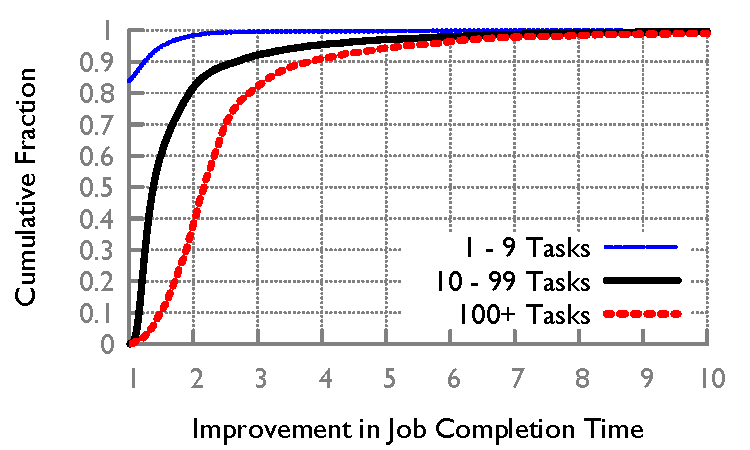
\includegraphics[width=0.45\textwidth]{figures/binpacked1-sep}
\vspace{-1.5in}
\label{fig:binpacked}
}
\hspace{0.2in}
\subfigure[] {
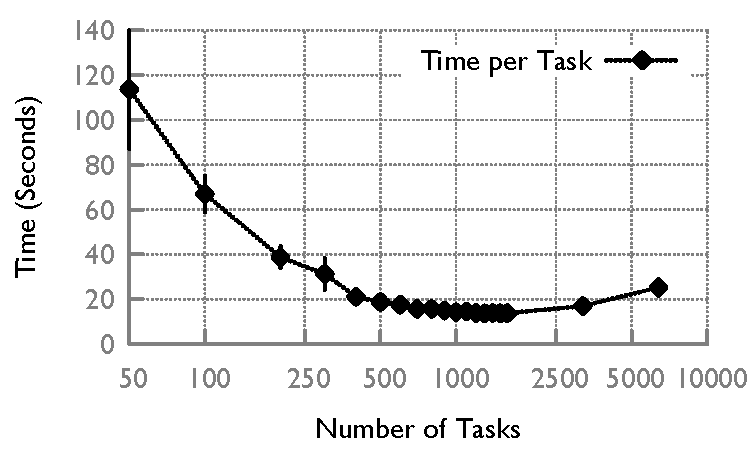
\includegraphics[width=0.45\textwidth]{figures/spark-skew-results}
\vspace{-1.5in}
\label{fig:sparkskew}
}
\caption{\subref{fig:binpacked} Improvement from perfectly balancing the total machine time for the
job across tasks. \subref{fig:sparkskew} Improvement from using tiny tasks in a cluster where 20\% of machines
take 21x longer to run each task. Error bars depict standard deviation.}
\vspace{-0.1in}
\end{figure*}

In this paper we present arguments and results motivating a move towards tiny tasks,
and we present preliminary design for a system supporting tiny tasks. In particular,
we propose a system that supports $100$ microsecond task launches, and an architecture
that allows most general applications to be expressed in terms of a set of tiny tasks.

\eat{We begin by quantifying the benefits of tiny tasks, using a series of simulations,
and application built on Spark\cite{zaharia2010spark} demonstrating the potential benefits
of using Spark. In Section~\ref{something} we outline the architecture for our system supporting tiny tasks, and
try and determine an appropriate task length based on task launch overheads, and other factors.
Next in Section~\ref{somethingelse} we discuss how to convert arbitrary jobs to better take advantage of tiny tasks, following
hich we discuss related work in Section~\ref{something}. Finally we conclude in Section~\ref{conclusion}.}

\section{Benefits of Tiny Tasks}

\label{sec:benefits}

Tiny tasks benefit datacenter workloads by reducing scheduling quanta. Using
a trace-driven simulation and experiments with Spark~\cite{zaharia2010spark},
we demonstrate that tiny tasks can improve job response times by
as much as a factor of 5.2.

%Tiny tasks benefit datacenter workloads by increasing the amount of elasticity
%available to the scheduler: tiny tasks occupy resources for a very small
%duration, so resources can be allocated at a very fine time-granularity. This
%allows resources to be dynamically reallocated between jobs, enabling greater
%cluster utilization without sacrificing request latency, and allows
%resources to be dynamically
%reallocated between tasks within a job, eliminating problems caused
%by straggling tasks and data skew.

\subsection{Handling of Skew and Stragglers}

\begin{figure}[t]
\centering
\subfigure[Today's tasks] {
    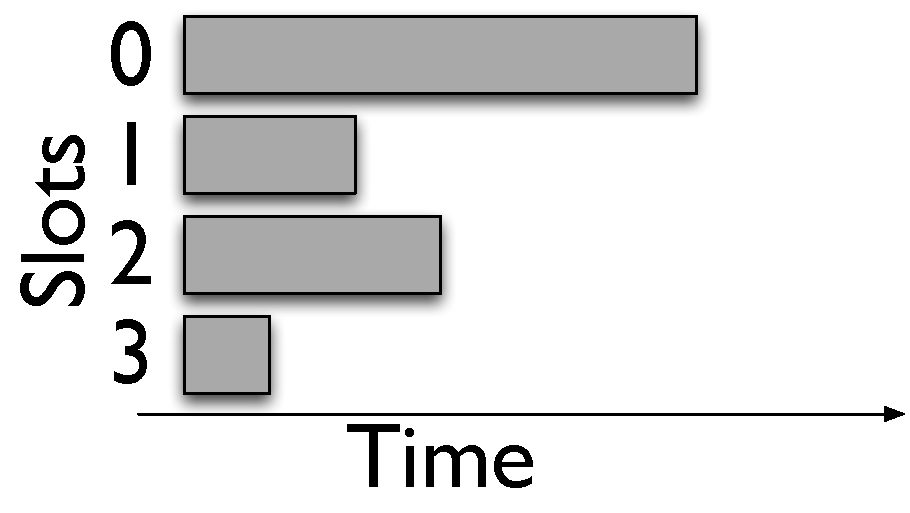
\includegraphics[width=0.21\textwidth]{figures/binpacking-before}
    \label{fig:tiny_diagram_original}
}
\subfigure[Tiny tasks] {
    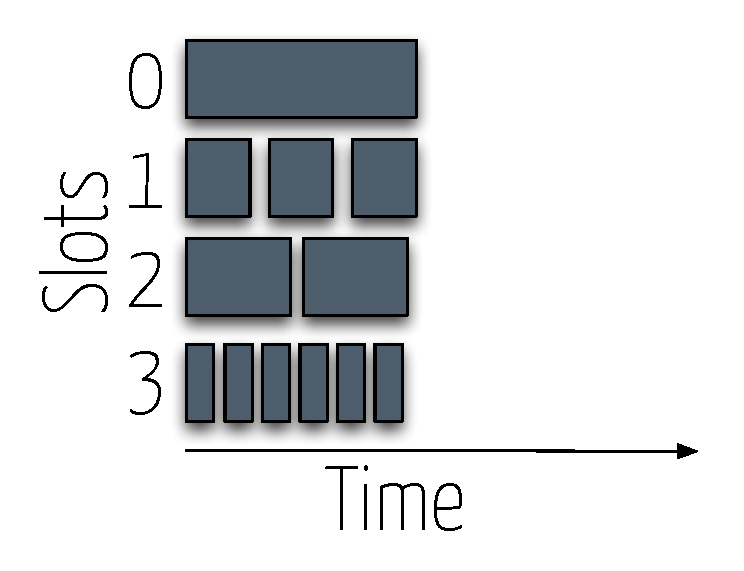
\includegraphics[width=0.2\textwidth]{figures/binpacking-after}
    \label{fig:tiny_diagram_tiny}
}
\vspace{-0.1in}
\caption{Tasks for a single job in a 4-slot cluster.
With tiny tasks, work is allocated to machines at fine
time-granularity, mitigating the effect of stragglers and allowing
the job to complete more quickly.}
\vspace{-2ex}
\label{fig:tiny_diagram}
\end{figure}


\begin{figure}[t]
  \centering
    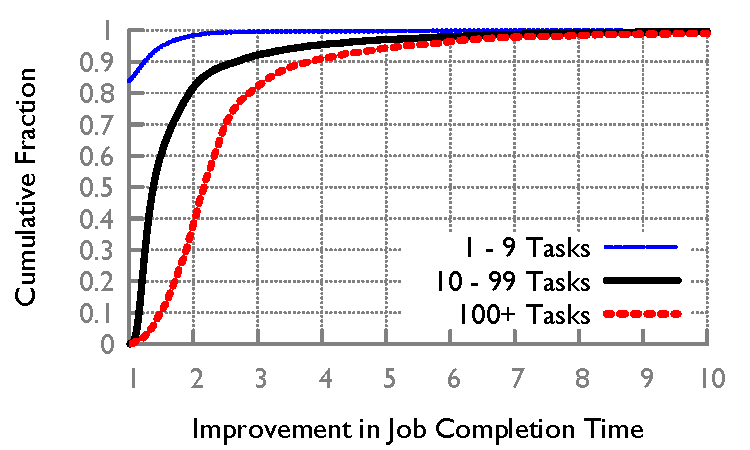
\includegraphics[width=0.4\textwidth]{figures/binpacked1-sep}
    \vspace{-3ex}
    \caption{ Improvement from perfectly balancing the total machine time for
    each job across its slots. Jobs that originally had more tasks see
    a more substantial improvement because having a large number of tasks increases the
    likelihood that the job includes stragglers.}
    \label{fig:binpacked}
\end{figure}

\begin{figure}[t]
\centering
    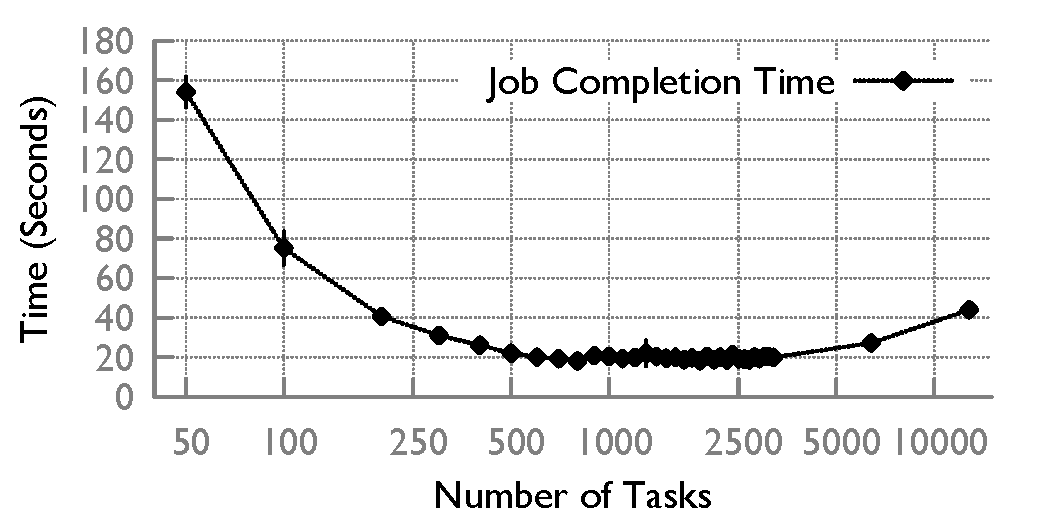
\includegraphics[width=0.45\textwidth]{figures/spark_experiment/straggler}
    \vspace{-3ex}
    \caption{Completion time for a Spark job that is split into various numbers of tasks. The job is executed in a cluster where 20\% of machines
take 20x longer to run each task. Error bars depict standard deviation.}
    \label{fig:sparkskew}
\end{figure}
Prior studies~\cite{ananthanarayanan2010reining,zaharia2008improving} have
noted that job response times in data parallel workloads tend to be
dominated by straggler tasks that take much longer than other tasks in the
job to complete.
%have noted that
%task lengths in data parallel workloads are highly variable and that outlier
%tasks negatively impact job completion time.
These outliers occur for one of two reasons.
First, outliers may be caused by poorly performing machines that cause tasks scheduled
on them to take longer; e.g.,
due to malfunctioning disks, contended CPUs, or congested networks.
Second, work may have been unevenly
divided across tasks, either due to
partitioning skew, where data was unevenly allocated to tasks, or due to
computational skew, where some data is more expensive to process.

Tiny tasks transform both the slow resources and the data skew problem
into a scheduling problem.  Rather than needing to predict which resources
are slow or statically partition data across tasks, a job is divided into
thousands or millions of sub-second tiny tasks, and each task is scheduled
as resources become available (shown in Figure~\ref{fig:tiny_diagram}).  In this manner, work is automatically
distributed evenly over available resources, without requiring complex skew
mitigation techniques: if a machine runs a computationally expensive task, it
will simply be assigned fewer total tasks.  Similarly, slow resources will
automatically be assigned less of a job's work, without needing to predict which
machines will perform poorly.

\eat{
Tiny tasks help mitigate the effect of outliers in two ways. First, splitting
total work across a larger set of tasks more evenly partitions records across tasks, reducing data skew;
secondly, individual tasks can be moved in response to slow machines, network congestion, or
other cluster conditions, and run on other, faster machines.
}
We use a Facebook trace~\cite{chen2012interactive} to quantify how much job response time would
improve if work were perfectly partitioned across machines.
% evenly distributing work over available
%resources, we used a Facebook trace to determine how much
%job response time would improve if work were perfectly partitioned across
%machines.
The trace contains 54,976 jobs.
For each job in the trace, we ask how long the job would have taken if the
total time for all tasks in the job were perfectly divided over the slots
used by the job.
Figure~\ref{fig:binpacked} compares this binpacked completion time to the
job's original completion time. Evenly balancing work improves performance by
$2.2$x and $5.2$x at the median and 95th percentile, respectively, for
jobs that originally had 100 or more tasks.
%Jobs that originally had
%100 or more tasks benefit substantially from balancing work more evenly:
%the median and 95th percentile reduction in completion time is $2.2$s and
%at the median, large jobs see
%For each job, we divided the total runtime for all tasks in the
%job by the average number of slots used and compare this time to the job's
%original completion time.
%Our experiment studies the benefits of perfectly balancing
%work across machines; with tiny tasks, two machines may differ in the amount of
%time spent processing data for a particular job by as much as one task
%length.
%Figure~\ref{fig:binpacked}
%demonstrates that jobs with 100 or more tasks benefit substantially from
%balancing work more evenly: at the median, large jobs see
%a $2.2$x reduction in response time from evenly spreading load
%across machines, and
%jobs at the 95th percentile see a $5.2$x reduction in response time.
This experiment provides a conservative bound on the speedup for two reasons. First, jobs
may have been using fewer than their fair share of slots in the original trace,
simply because there were not enough tasks to occupy more slots; in this case,
tiny tasks will further improve performance by increasing parallelism. Second,
if a task is running on a slow machine, it may take less total time when
broken into tiny tasks, because some of the tiny tasks will be run on faster
machines.
This experiment underestimates the possible improvements from
evenly balancing work but ignores task launch overheads, which
we address in the next experiment.
%However, we note that this simulation ignores any overheads associated with
%tiny tasks and we measure the effects in our next experiment.


\eat{Figure~\ref{fig:sparkskew} demonstrates the improvement offered by tiny tasks on a Spark MapReduce job with data skew and machines that exhibited a random 5x performance variance.
With tiny tasks, Spark is able to mitigate both skew and stragglers without explicit knowledge of machines' speeds or records' processing costs.}

%Next, we use Spark~\cite{zaharia2010spark} to demonstrate that tiny tasks
%improve performance in the presence
To demonstrate that using tiny tasks improves performance in
the presence of slow machines,
we modified some machines in a cluster to run more slowly, and then
ran a Spark~\cite{zaharia2010spark} job using different numbers of tasks.
We used $50$ m1.medium EC2
instances, 10 of which were modified to take 20x longer to run each task.
Figure~\ref{fig:sparkskew} demonstrates that using a larger number of tasks
improves response time by 8x compared to using the same number
of tasks as machines in the cluster, because the slow machines are
\eat{assigned approximately $\frac{1}{20}$ as many tasks}assigned fewer tasks. Beyond $2000$ tasks, task launch overheads cause increased response time; we discuss
how to decrease overheads in \S\ref{sec:sched}.

%\begin{figure*}[!ht]
\begin{figure}[t]
\centering
\subfigure[Today's tasks] {
    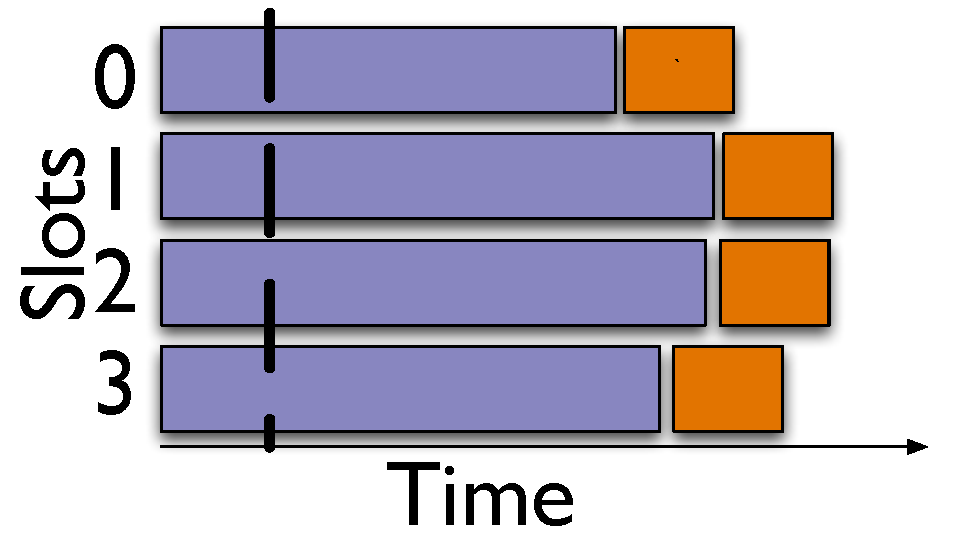
\includegraphics[width=0.22\textwidth]{figures/slot_diagram_after}
    \label{fig:slot_diagram_original}
}
%\hspace{0.5in}
\subfigure[Tiny tasks] {
    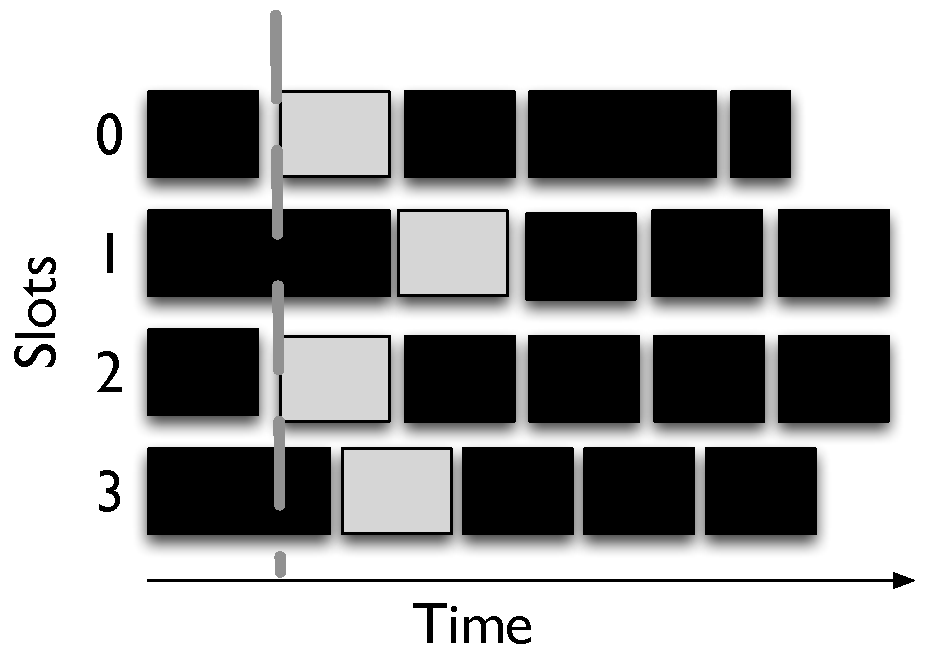
\includegraphics[width=0.22\textwidth]{figures/slot_diagram_before}
    \label{fig:slot_diagram_tiny}
}
\vspace{-0.1in}
\caption{
A high priority dark job arrives (at the dashed line) in a cluster where all
slots are in use by a low priority light job.
%    The dashed line denotes the arrival of a a high priority (dark) job
%in a cluster where
%all 4 slots are in use by a low priority (light) job.
%Two jobs running in a cluster with four slots.
With today's tasks,
tasks for the high-priority job must wait for long-running tasks from the light job to
complete before being launched.
With tiny tasks, resource
allocation is fine-grained, so resources will quickly be allocated to
the higher priority job.}
%new
%jobs, allowing the higiher-priority grey job to complete more quickly.}
\vspace{-2ex}
\label{fig:slot_diagram}
\end{figure}


\subsection{Improved Sharing}
Today, sharing a cluster between interactive and batch jobs involves trading off
responsiveness and utilization. If a cluster is highly utilized,
an interactive job may need to wait for long-running batch tasks to
complete before it can be serviced; reserving slots for
interactive jobs avoids this problem but results in lower utilization.
Using tiny tasks for all jobs avoids this trade off: the cluster can run at
high utilization, while
simultaneously guaranteeing that interactive jobs will only need to wait for
a short time before being serviced. Figure~\ref{fig:slot_diagram} depicts a simple example
with only two jobs, and demonstrates that with tiny tasks, a newly arriving
job can quickly obtain resources, even in the presence
of batch jobs.

\section{Architecting for Tiny Tasks}
Tiny tasks present many design challenges for computing frameworks.
Splitting jobs into tiny execution units requires low-overhead
high-throughput scheduling, scalable storage systems and a programming model
that can be used to support different kinds of computations.
% TODO(josh): maybe the bit about "different kinds" can be made clearer?
In this section, we present our design goals and outline the challenges in
realizing them.
% TODO(josh) Do we need this transition sentence?

\subsection{Execution Model}
We propose an execution model where every job in the cluster is split into a
large number of tiny tasks. Similar to existing frameworks, each task is a
deterministic unit of execution and a task's description contains the code to be
executed and a set of named inputs chunks. We enforce that each input chunk is
restricted in size to 8MB and that tasks execute in around $100$ms.  Unlike
existing systems, our task execution framework pre-fetches a task's input into
memory (Section~\ref{sec:pipeline}) before running it. Tasks produce a set of named
outputs that can be used as inputs by subsequent tasks. We use a co-operative
multi-tasking scheme where the scheduler waits for a task to finish before launching
the next task.  Task running times are controlled by using small input blocks
and support from programming frameworks. We compare against alternate design
schemes in Section~\ref{sec:alternate}.

\subsection{Low-latency scheduling}
In a datacenter containing thousands of machines, having tasks which execute for
$100$ms would mean that cluster schedulers need to make millions of scheduling
decisions every second. Centralized scheduling schemes have well-known
scalability limits~\cite{john-wilkes-berkeley} and distributed scheduling
schemes will be required to handle tiny tasks. Recently proposed distributed
scheduling techniques like batch sampling~\cite{sparrow} have been shown to
provide near-optimal scheduling decisions. We plan to explore distributed
scheduling schemes which can also provide fairness guarantees and balance
utilization of machines across the cluster. To minimize data-movement
schedulers will also have to consider locality constraints
and techniques like delay-scheduling~\cite{delay} can be used to maximize locality at the
cost of latency.

In addition to scheduling latency, task launch overheads will have to be
minimized to ensure that tasks can spend a large fraction of their execution
time doing useful work. Existing frameworks like Hadoop typically launch a new
JVM for each task and launching new tasks takes \fixme{5-10} seconds. Newer
frameworks like Spark reuse existing JVMs, but task launch overhead is still on
the order of a few milliseconds~\cite{sparrow}.

We believe that average task launch overhead can be reduced $100 \mu$s, making it
an insignificant portion of the execution time. Much of the existing task launch
overhead stems from shipping the task over the network and this can be
eliminated by caching tasks. Task launch latency can then be reduced to one
intra-datacenter RPC, containing a checksum of the task description, path to
task inputs, and the time required to execute a new thread. Furthermore, 
scheduling decisions where a task continues to execute in a given slot can be 
efficiently implemented using a lightweight renewal message similar to leases.\\

\subsection{Pipelined Execution}
\label{sec:pipeline}
Task execution can be made more efficient by using a pipelined execution scheme.
Every tiny task can be broken down in to three main phases: a fetch phase where
the task descriptions and the inputs are fetched consuming I/O resources, an
execute phase where task consumes CPU and an output phase where the tasks
outputs are saved to the storage system. By pipelining CPU and I/O resources
across different tasks, we can further reduce associated overheads. With tiny
tasks we expect task inputs and outputs to be small as well and this allows the
execution framework to cache these values and flexibly schedule data transfers.
Using a data transfer interface similar to coflows~\cite{coflow-hotnets} we
believe that explicitly managing data transfer between tasks will allow us to
optimize network utilization in the data center.

\subsection{Scalable Storage Systems}
In order for tasks to be short, they must operate on a small amount of on-disk
data, or use in-memory data.  For data stored on-disk, assuming data can be read
from disk at 100MB/s, a task can read no more than 10MB of data in 100ms.  Hence
we propose that blocks in the distributed file system must be limited to around
8MB. Existing file systems like HDFS, which use a centralized metadata server,
hit scalabilty limits with smaller block sizes~\cite{facebook-berkeley-talk}.
Recent work on Flat Data Center Storage~\cite{fds}, addresses this problem by
distributing metadata across servers and their results indicate that tasks can
overcome the need for disk locality. While FDS provides a natural environment
for tiny tasks, we believe there is a need to consider in-memory locality as
well. Accessing in memory data~\cite{pacman, spark} will enable tasks to access 
up to 1GB in 100ms and an integrated approach to caching, scheduling based on
memory locality and appropriate placement on disks will be necessary to handle
tiny tasks.

\subsection{Programming model}
\label{sec:prog}
Splitting jobs into tiny tasks is relatively straightforward for data parallel
programs as programming frameworks can sub-divide the input to many more tasks.
However some computations could become more expensive as we increase the total
number of tasks. An example of this would be MapReduce computations where we
have an all-to-all shuffle ($O(N^2)$ in communication) and benefits from higher
degree of parallelism may not enough to offset the costs. Combiners, which can
perform partial aggregation of data, are commonly used in computations which are
associative and commutative. Extending this, we plan to explore using
aggregation trees~\cite{something} which can address this problem and ensure
that tasks remain tiny.

However we could still have computations that are either not associative and
commutative or require a large amount of temporary state (e.g. computing
distinct elements). To handle such computations, we propose providing 
support for a distributed ``scratch space'' that can be used by tasks to 
communicate across different executions. For example, to compute the set of
unique elements in a file, tasks could use the scratch space to store elements
seen so far. We envision that a simple key-value store like interface would
be sufficient for this purpose and plan to provide strong 
consistency~\cite{something} for accesses within a datacenter. 

As an exception, we also plan to accomodate some large tasks in the cluster.
This would require programmer intervention to explicitly annontate such tasks
and scheduler modifications will be necessary to support this hybrid model.  As
large tasks have been shown to occupy most of the cluster's
resources~\cite{something}, we plan to explore the trade-off between flexibility
and utilization while supporting larger tasks.  While the projected benefits of
using tiny tasks (Section ~\ref{sec:benefits}) are realized when all the tasks
are uniformly small, we believe that supporting a few large tasks will still
provide significant benefits.

\eat{
- Major point: Data intensive applications have a lot of state -- and
this is hard to checkpoint. Need a crisp quantitative argument for
this.
- Lots of work in distributed OS about this - Amoeba, Sprite, Chorus
etc. Also VM migration work. Need to differentiate from them.
- Argue for global scheduling as we want load balancing across the datacenter.
}


\eat{
\subsection{Low-Overhead Scheduling}
Breaking each task into hundreds or thousands of tiny tasks leads to 2-3 orders
of magnitude more scheduling decisions that the scheduler needs to make.
While the Hadoop job tracker (for example) has a well-known scalability limit
at approximately 4000 machines, recent work~\cite{sparrow} has shown that
distributed scheduilng provides a near-optimal and highly scalable alternative
to centralized schedulers. Might also want to cite YARN here, even though it
does not work as advertised.

Can use leases to further improve scalability.

Early frameworks (e.g., MapReduce) launch a
new JVM for each task, so launching a task takes seconds.  Earlier
work~\cite{Amoeba} has used high task launch overheads to argue against
using smaller task sizes.  Launching a new JVM for each task is
unnecessary and costly; newer frameworks like Spark don't do this and can
launch tasks in milliseconds (true?).

\subsection{Scalable File System}
In order for tasks to be short, they must operate on a small amount of on-disk
data, or use in-memory data.
For data stored on-disk, assuming data can be read from disk at 100MB/s,
a task can read no more than 10MB of data if it is to complete in 100ms.
Current file systems like HDFS already hit scalabilty limits in many clusters
using the default block size of 64MB (Facebook uses 1GB block sizes for this
reason), so could not handle the metadata needed to store small file blocks.
The recent Flat Data Center Storage~\cite{fds} work solved this problem
by distributing meta data in the magic table; tiny tasks would be built
atop a file syste like FDS.

To make tasks complete even faster, tasks may operate on in-memory data.
Frameworks like Spark and PacMan store disk in memory, allowing a task that
completes in 100ms to scan as much as 1GB of data.

Comment on memory: we anticipate needing some degree of locality, unlike FDS,
since there will always be a storage technology with higher bandwidth than
is current cost effective for networking. Scheduling in this environment
is an open problem but might rely on something like delay scheduling, which
can be implemented in distributed schedulers (see Sparrow).

\subsection{How Low Can We Go? (move this throughout!)}
Given the architecture described above and current technologies, we expect that
running tasks shorter than 100ms will lead to significant overheads. With disk
blocks lower than 8MB, can no longer amortize seek times, making disk reads take
longer. (use progress rate graphs to show what task lengths this would lead to?)

We are hopeful that storing data in memory and further
improving scheduling can drive task launch overheads to <1ms, making tasks that
complete in tens of milliseconds practical.

\subsection{What About Tasks that Cannot Easily Be Parallelized?}
As a starting point, we consider the improvements from ``tiny-ifying'' only the
tasks that are easily parallelized.  Figure~\ref{??} depicts the performance of
tiny tasks as we decrease the percentage of tasks that can be parallelized, based
on traces from Facebook.  There is an elbow at ??.

As shown in Figure~\ref{??}, using tiny tasks as a design principle improves
performance by X\%, but when tasks cannot be parallelized, we leave X\% of
performance on the table.  To enable making \emph{all} tasks tiny, we propose
creating a new computing framework that provides distributed ``scratch space.''
Parallelize by storing some stuff in this scratch space, so it can be accessed
by multiple tasks.  Give an example (e.g., unique). Provide some estimate
of how many tasks fall in this category?
}

\section{Alternate Designs and Related Work}

Tiny tasks solve two major problems in data centers: outliers, and sharing
a cluster between batch and interactive or user-facing jobs. A variety of
approaches solve one of the two problems in isolation; e.g., skew handling
techniques mitigate outliers, and process migration allows improved
sharing between long and short jobs.  Unlike these approaches, tiny tasks
provides a simple design paradigm that solves both problems.

\subsection{Preemption and Process Migration}
%\subsection{Alternate Design Schemes}
\label{sec:alternate}

Our choice of a cooperative multi-tasking scheme is in contrast to
preemption based schemes commonly used in operating systems. The benefits of 
preemption and short quanta are well studied in operating
systems literature; for instance~\cite{sherman1972trace} shows the benefits
of short scheduling quanta. A large body of work in distributed 
operating systems~\cite{douglis1991transparent,milojivcic2000process,rozier1991overview} and virtual machines~\cite{tanenbaum1990experiences}
has applied preemption in a distributed context by exploring migrating
processes between machines.
We find that preemptive mechanisms are
ill-suited to data parallel jobs running on a cluster as discussed below.\\
%However achieveing low overhead task-switching is more expensive in the distributed setting. 
\textbf{Cost of task-switching}: Work on process
migration~\cite{douglis1991transparent,milojivcic2000process} and virtual
machine migration~\cite{clark2005live} has shown mechanisms to transparently
move tasks across machines. Such methods however involve a high overhead, as
migrating a task involves transferring both task context, a tasks intermediate
data, and its inputs. For data parallel applications, input data, and intermediate
data can be several gigabytes, incurring very high overheads.

Cooperative multitasking by contrast eliminates the need to migrate such data. In
addition we envision moving shared state into a framework maintained scratch space,
by explicitly differentiating such state, we envision it can be more easily migrated.

\textbf{Fault tolerance:} In a datacenter setting, tiny tasks are better suited for
fault tolerance when compared to task preemption. Since each tiny task is a
deterministic unit of work, tasks can be executed in parallel during recovery.
In contrast, using preemption one would need to maintain redundant checkpoints
and fault recovery cannot be executed in parallel. \\

\textbf{Enforcing tiny tasks:} Preemption allows a framework to finely control
task lengths. However controlling task inputs, and minor modifications to the 
framework will ensure that all tasks are short.

Recent work proposed Amoeba~\cite{ananthanarayanan2012true}, a system that identifies safe points in MapReduce-style
jobs where a task can be migrated. At safe points, a task can checkpoint its
output and a new task is spawned to process remaining inputs. The Amoeba authors
choose preemtability rather than small tasks because they note that creating
\emph{uniformly} sized small tasks is difficult. We emphasize that tasks need
not be unfiformly sized to see the benefits of tiny tasks; task lengths
should generally be sub-second, but may span 2-3 orders of magnitude.
Furthermore, while Amoeba allows better sharing of batch and interactive
workloads, it does not mitigate skew or outliers.

\subsection{Static Partitioning}
Omega, Google's newest cluster scheduler~\cite{melnik2010dremel},
was designed to share cluster
resources between batch and interactive workloads. However, Omega achieves
this by
statically partitioning cluster resources.  
Interactive services like Dremel~\cite{melnik2010dremel} spin up long-running
agents that serve incoming queries, rather than scheduling new resources for
each request.  Static partitioning limits utilization because each service
must be provisioned to handle peak load, and one service's extra capacity
cannot easily be reallocated to another service.

\subsection{Skew-Handling}
A separate line of research has focused on skew-mitigation to improve job
performance in datacenters. Examples of such work include
Mantri~\cite{ananthanarayanan2010reining}, SkewTune~\cite{kwon2012skewtune},
Scarlett~\cite{ananthanarayanan2011scarlett}, and work on task
speculation~\cite{zaharia2008improving}. Mantri and Scarlett attempt to
mitigate task runtime skew by modeling the causes for skew and accounting for
these causes when scheduling tasks. In particular Mantri performs resource aware scheduling to decrease the
probability of observing task skews, while Scarlett replicates storage blocks
based on their probability to decrease the wait time for a popular block. While
both of these systems moderately reduce task skew, they rely on a fragile set of
signals, and do not work in all cases. Using tiny tasks naturally overcomes data
skew among reduce tasks as fine-grained hash partitioning ensures that the data is
more evenly spread across tasks. As shown in 
Section~\ref{sec:benefits}, using tiny tasks also allows work to be balanced across
different machines thereby overcoming skew due to slow machines.
Furthermore, existing skew mitigation techniques trade-off cluster resources to
gain more predictable task runtimes. This limits the applicability of these
techniques under situations of high load, where such guarantees might be most
important.


%\section{Related Work}

There has been a large body of work in the context of distributed operating 
systems~\cite{douglis1991transparent, milojivcic2000process, amoeba-os, chorus} 
and virtual machines~\cite{xen, something} that have looked at scheduling and
context-switching among processes across different machines. Migration of
processes or virtual machines typically use premptive methods and we compare
them to our design goals in Section~\ref{sec:alternate}.

Recent work proposed Amoeba~\cite{ananthanarayanan2012true}, a system that
shares similar goals as our work. In Amoeba, the system identifies safe-points
where a task can be killed, while minimizing wasted work. At safe-points a task
can checkpoint output based on inputs it has processed so far, and a new task is
spawned to process the remaining inputs. This work is perhaps closest to
TinyTasks, and shows that preemptibility is an important feature for tasks
scheduled on a cluster.  However, while the work acknowledges the necessity for
preemptibility, it places no requirements on how frequently safe-point occur,
and hence places no bounds on the maximum time for which a single task can
capture the processor.  Furthermore, actually determining safe-points for
general tasks is non-trivial, and while Amoeba provides some examples of
safe-points for certain kinds of tasks, they do not provide a generic framework
for determining where such safe-points could occur.  TinyTasks by contrast do
not require any program analysis to identify such points, and instead relies on
limiting input sizes to achieve preemption.

Dremel~\cite{melnik2010dremel}, in conjunction with Google's cluster scheduler
Omega~\cite{wilkes-berkeley}, has also been used to run interactive jobs in a
cluster otherwise used for batch processing. Dremel achieves low latency by
spinning up long-running agents on which queries are executed. This is similar
to statically partitioning a cluster, where a part of the cluster is reserved
for interactive jobs, and the rest can be used for batch jobs. Such a method
necessarily limits the utilization of a cluster, and requires that the peak load
for interactive jobs be known in advance, so as to ensure that constraints are
met. Requiring application requirements be known in advance makes static
partitioning unsuitable to shared clusters with frequently changing workloads.

\eat{\paragraph{Process Migration} Include operating systems work on process
migration, as well as Ganesh's Amoeba paper. This work is most similar to
our approach. With tiny tasks, we are effectively architecting for pre-emption,
without needing to worry about moving large amounts of contexts between a
stopped and re-started job.

\paragraph{Skew Mitigation} Large body of over-engineered work on skew-
mitigation; most solutions fix only part of the problem and are highly
complex

\paragraph{Running Batch Workloads Alongside Interactive Workloads}
Google touts the fact that Omega/Borg schedule for both batch and interactive
workloads, but what they do is effecitively static partitioning (interactive
services have some portion of the cluster that they re-use to execute requests,
rather than scheduling a new job for each user request)! E.g., 
Dremel has a statically allocated part of the cluster.}

\eat{
The benefits of preemption and short task length are well studied in operating
systems, for instance~\cite{sherman1972trace} shows that operating system
schedulers should ideally be preemptive, and should prevent jobs from capturing
the CPU for too long a time. This is unfortunately harder to achieve in the
cluster computing context, since resource allocation includes much more than the
CPU, and revoking allocated resources might require moving the task. Previous
work has also looked into process
migration~\cite{douglis1991transparent,milojivcic2000process}, where processes
are transparently moved between machines. These methods present overheads, as
process context and state needs to be transfered across the network. For large
tasks such state can be of significant size, and such transfer would put a
significant load on the data center network. 
}

\section{Conclusion}
%We have described the great benefits of having tiny tasks and no tradeoff.
%We believe that as system designers and cluster architects, we should 
%try to build systems that allow this goal to be realized.
%We have described an initial architecture and some of the components
% that we think are requiredas the first steps twoards this goal.
Tiny tasks represent a simple design change that mitigates stragglers and
allows increasing utilization without sacrificing fairness or responsiveness.
We have presented an architecture that represents a first
step towards realizing tiny tasks.
Our work highlights the importance of efforts to reduce overheads and provide
increased scalability in cluster frameworks.
%Given the benefits of using smaller tasks, we believe that the systems
%community should focus on efforts to reduce overheads and provide
%improved scalability in cluster frameworks.


\bibliographystyle{abbrv}
\bibliography{tiny-tasks}

\end{document}
